\begin{frame}{Интеграция AlgoView в систему AlgoLoad}

Одна из приоритетных областей использования системы визуализации — помощь в образовательных программах. 

\vspace{5mm}

Например, AlgoLoad — одна из студенческих платформ контроля рассылки и сдачи заданий на факультете ВМК МГУ. В 2023 году AlgoView была интегрирована в AlgoLoad взамен устаревшей системы визуализации.

% В ходе работы над обновлением системы AlgoLoad были произведены следующие действия:

% \begin{itemize}
%     \item Технологическая платформа AlgoView установлена взамен старой;
%     \item Обновлен способ передачи и обработки пользовательского файла конфигурации графа;
%     \item Изменен способ передачи файлов визуализации на сторону клиента; 
%     \item Добавлены методы логирования процесса обработки и передачи данных;
%     \item Оптимизирован метод хранения пользовательных данных;
%     \item Исправлено множество старых ошибок системы;
% \end{itemize}

\end{frame}


% длинное тире: —


\begin{frame}{Анализ кодовой базы AlgoLoad (осень 2024)}
\begin{itemize}
    \item Устаревший код: На платформе AlgoLoad накоплен объем наследуемого кода, усложняющий модернизацию.
    
    \item Снижение качества: Устаревшая архитектура приводит к снижению адаптивности и надежности системы.
    
    \item Технический долг: Накопленный технический долг увеличивает затраты на обслуживание и ухудшает качество.
    
    \item Переработка кода: Предлагается частичная переработка кода для оптимизации работы системы.
    
    \item Использование Flutter: Рефакторинг на Flutter обеспечит более масштабируемое решение для фронтенда.
    
\end{itemize}
\end{frame}








\begin{frame}{Модернизация проекта}
\begin{itemize}
    \item Объединение страниц: Перенос всех веб-страниц студенческого функционала на одно Flutter Web приложение.

    \item Авторизация: Реализация сторонней авторизации для плавного перехода к новому функционалу.

    \item Динамическое изменение XML: Автоматическая подгрузка изменений структуры алгоритмов на странице задания.

    \item Интерактивные возможности: Реализация контекстного меню в 3D-визуализации графов.

    \item Оптимизация: Интеграция методов оптимизации для сокращения времени просчета нового графа через dart.ffi.
    
\end{itemize}
\end{frame}






 
\begin{frame}[fragile]{Внешний вид Flutter Web приложения}
% \vspace{2mm}
% 123

\vspace{3mm}
\centering
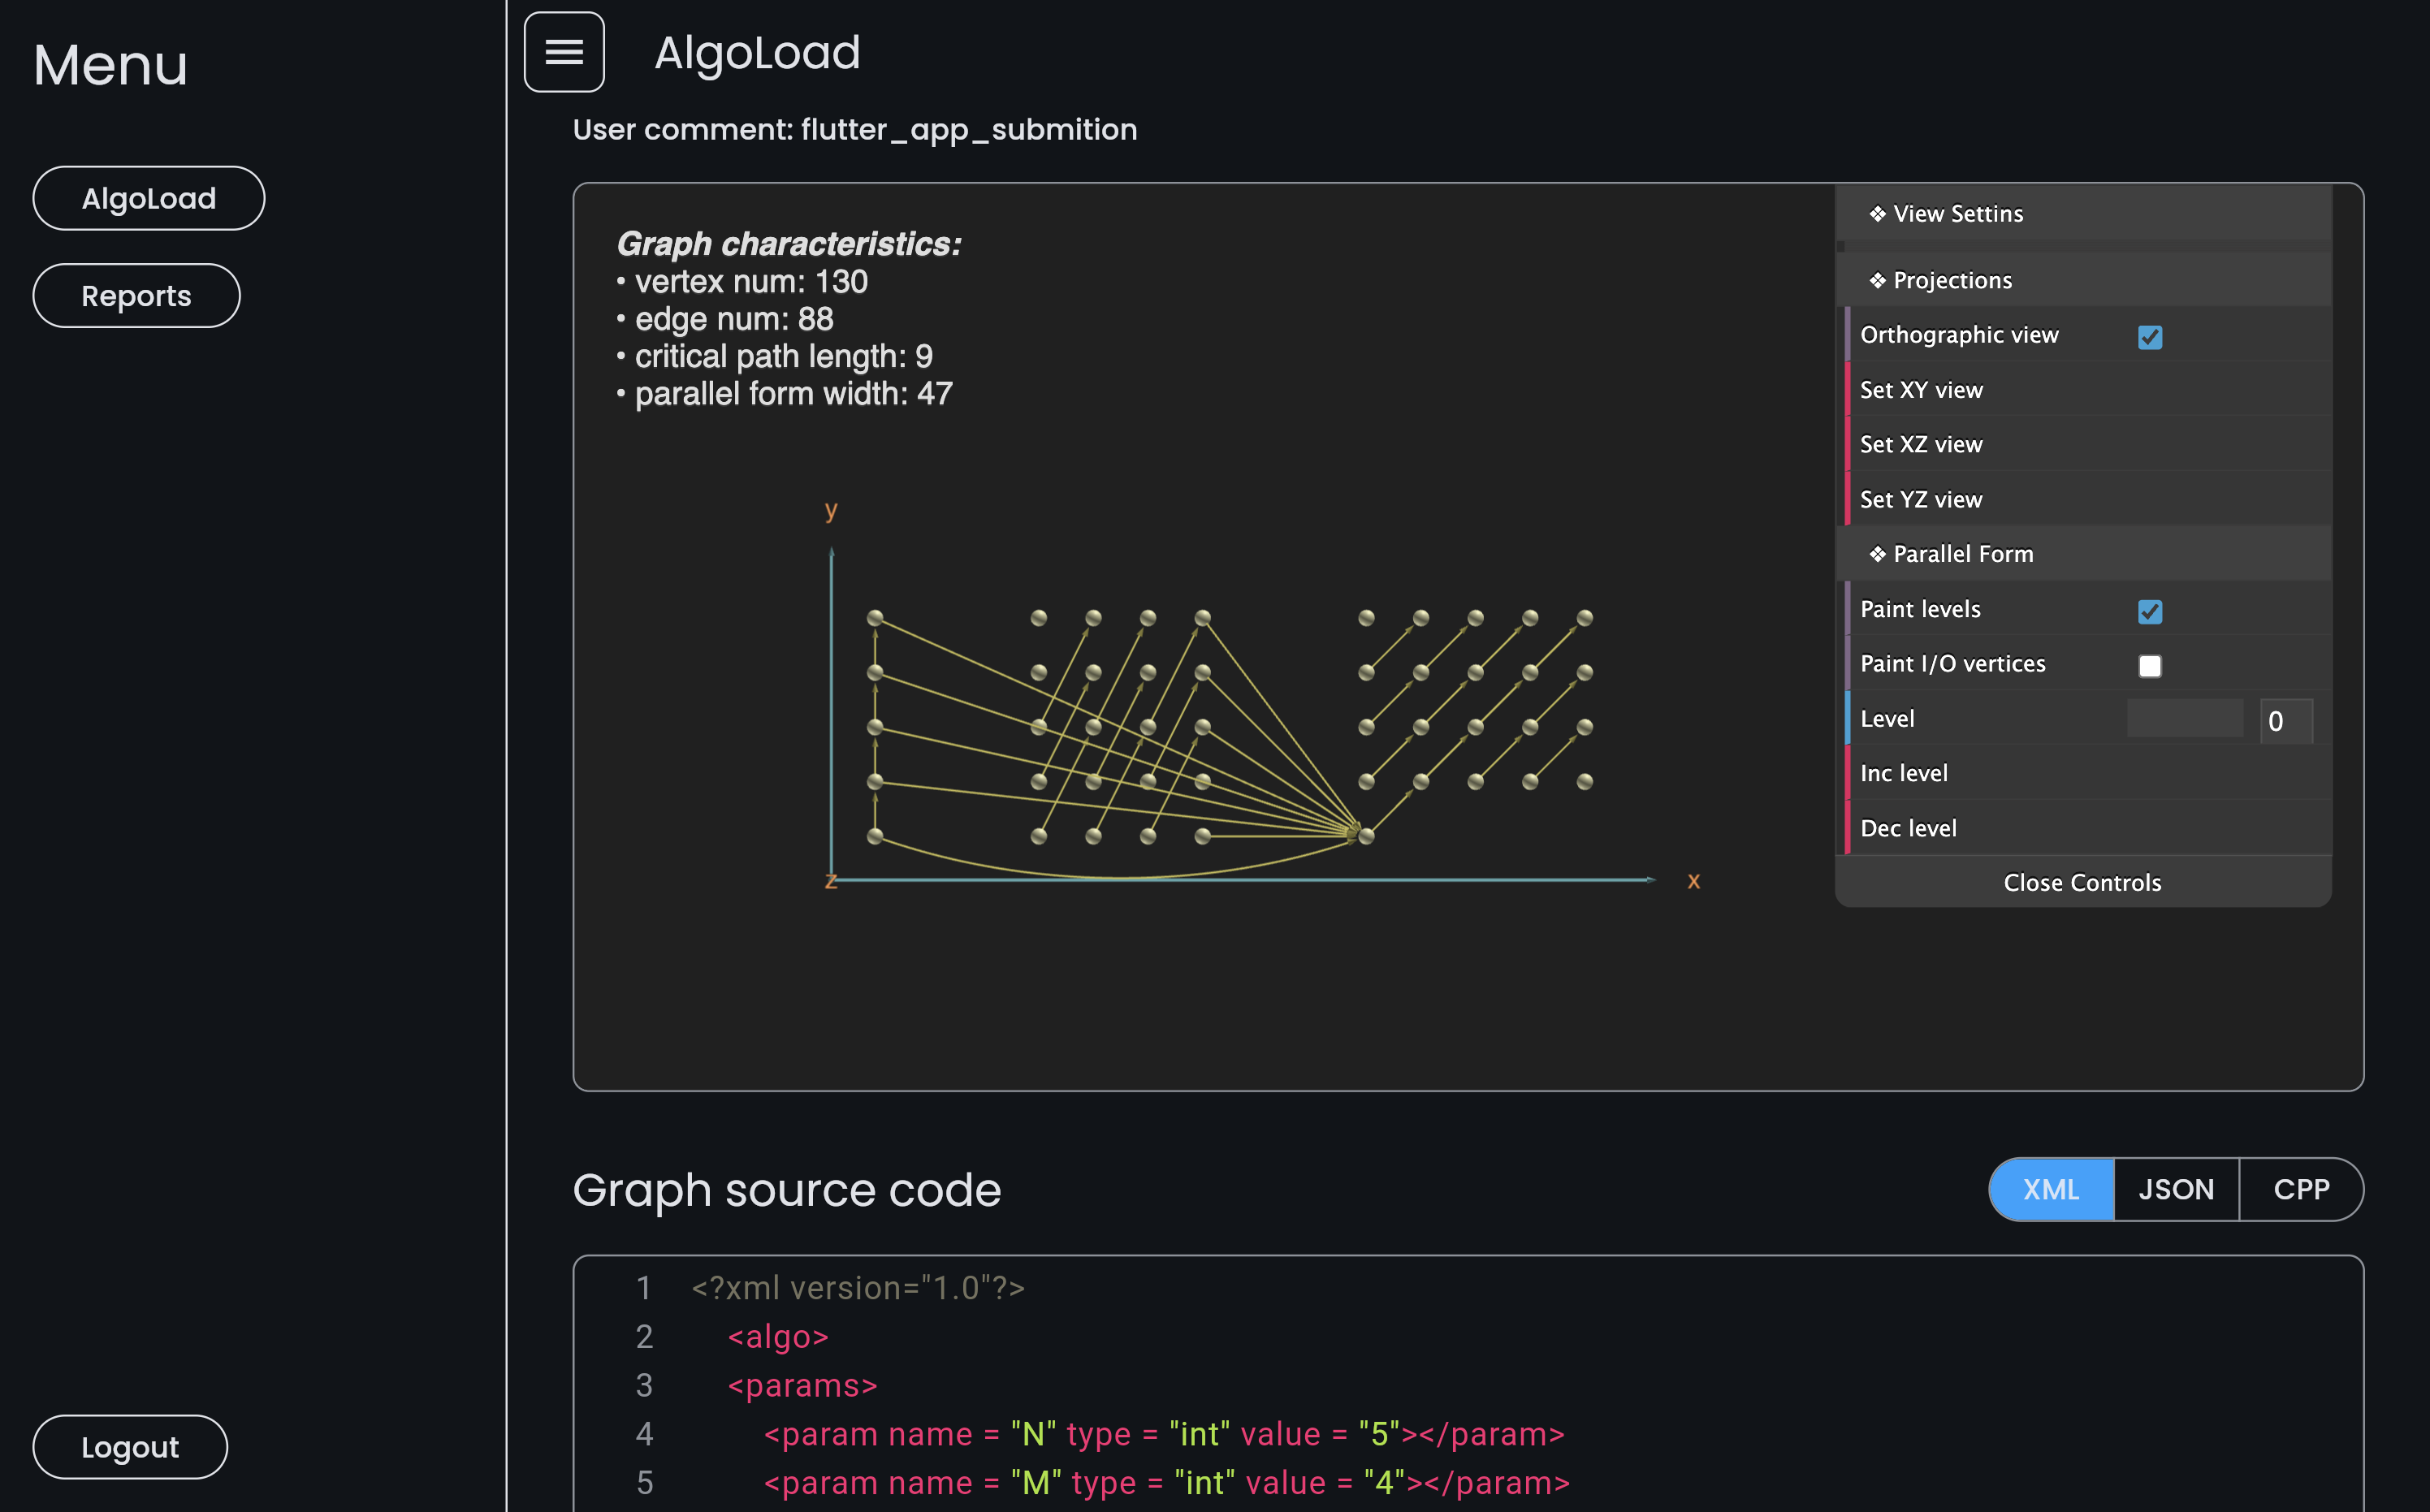
\includegraphics
[width=0.8\textwidth]{images/algoload_flutter_15_04_2025}\\

\end{frame}







\begin{frame}{Результаты работы}

\begin{itemize}
    \item Система AlgoView была разработана в соответствии с планом и является отличной платформой для изучения параллельных свойств алгоритмов, и удобным инструментом в руках исследователей;
    \item Система AlgoView была интегрирована в магистерскую учебную программу 6 курса на факультете ВМК МГУ и на протяжении 1 семестра работала безошибочно;
    \item Система AlgoView посредствам вывода ошибок и предупреждений позволяет эффективно работать и обучаться с подсказками;
    \item Проведена модернизация проекта в виде написания Flutter web приложения, с описанным выше новым функционалом.
    
\end{itemize}

\end{frame}
